\section{Smoothed Particle Hydrodynamics - Lagrangian Particle Method}
\thispagestyle{plain}
\idea{In Smoothed Particle Hydrodynamics (SPH) we approximately
solve the fluid equations numerically by replacing the fluid
with a set of particles, we call \textit{SPH-particles}\footnote{Characterized by their position and velocity. Additionally,
hydrodynamic variables, e.g. $\rho_i, T_i$, are derived at the particles positions $\vec{x}_i$. Not
to be confused with the real particles making up the fluid.}. The equations of motion and 
properties of those particles are followed from the Lagrangian form
of the continuity equations for the fluid. We then forward 
these particles in time using e.g. the leapfrog or semi-implicit
Euler scheme.}

From this it makes sense that the main ingredients to the baseline scheme will be
\begin{itemize}
    \item formulate the fluid equations in their Lagrangian\footnote{Co-moving with the flow rather than fixed as in the Eulerian perspective.} form
    \item formulate an algorithm to update the SPH-particles positions and velocities based on the Lagrangian fluid equations
    \item find expressions for the quantities used in the update-steps which goes hand in hand with finding how to get from the SPH-particle-perspective to continuous fluid quantities
\end{itemize}

Such a mesh-free scheme has \textcolor{green1}{some key advantages}
\begin{itemize}
    \item This particle representation of SPH has great conservation features - energy, linear momentum, angular momentum mass and specific thermodynamic entropy (more later; if we do not add artificial viscosity) are conserved (as we follow particles there is no loss of mass etc.).
    \item No advection errors, scheme is fully Galilean invariant (unlike mesh-based Eulerian techniques)
    \item As of the Lagrangian character, the local resolution of SPH follows the mass flow automatically $\rightarrow$ adaptive resolution, good for problems with vastly different densities
\end{itemize}

\subsection{Lagrangian fluid equations (i.e. as material derivatives)}
\subsubsection{Continuity equation}
Written as a material derivative, the continuity equation is
\begin{equation}
    D_t \rho = -\rho (\vec{\nabla} \cdot \vec{v}), \quad \text{fluid mass density } \rho, \quad \text{fluid velocity } \vec{v}
\end{equation}
which is zero for an incompressible fluid.

\subsubsection{Navier-Stokes equation | Conservation law of Linear Momentum}
A natural extension of Newtons 2nd law to continua is (including internal and external forces)
\begin{equation}
    \begin{gathered}
        \rho D_t \vec{v} = \sum \text{forces} = -\vec{\nabla} P + \vec{\nabla} \cdot \mat{\Pi} + \rho \vec{g} \\
        \text{stress tensor } \mat{\Pi}, \quad \text{pressure } P, \quad \text{external accelerations } \vec{g}
    \end{gathered}
\end{equation}
where a general approach to $\mat{\Pi}$ is the Cauchy-Stress tensor for compressible flow
\begin{equation}
    \begin{gathered}
        \mat{\Pi} = \left\{ \mu \left[ \vec{\nabla} \vec{v}^T + (\vec{\nabla} \vec{v}^T)^T - \frac{2}{3} (\vec{\nabla}\cdot \vec{v}) \mat{1} \right] + \zeta (\vec{\nabla}\cdot \vec{v}) \mat{1} \right\} \\
        \text{shear viscosity } \mu, \quad \text{bulk viscosity } \zeta
    \end{gathered}
\end{equation}

where for incompressible flow one yields

\begin{equation}
    \rho D_t \vec{v} = -\vec{\nabla} P + \mu \vec{\nabla^2} \vec{v} + \rho \vec{g}
\end{equation}

\note{In an incompressible setting, the pressure $P$ can be interpreted as a Lagrange multiplier which has to be chosen
such that incompressibility really holds. Otherwise $P$ is determined by a state equation, e.g. very basic $P(\rho) = k \left( \frac{\rho}{\rho_0} - 1 \right), k>0$ (variation of the ideal gas equation) or isothermal $P(\rho) = P_0 + c_0^2 (\rho_0 - \rho)$, as previously discussed.}

\subsubsection{Energy equation}
While me can forward the system only based on the Navier-Stokes equation and closure,
let us write down the energy equation.

Let $\epsilon$ be the energy per volume so the energy per mass is $e = \frac{\epsilon}{\rho}$.

From basic thermodynamics, we can write for the internal energy $U$

\begin{equation}
    \begin{gathered}
        dU = dQ + dW = dQ - PdV = T dS - P dV, \quad U = \epsilon V = eM \\
        \text{volume } V = \frac{M}{\rho} \rightarrow dV = -\frac{M}{\rho^2} d\rho, \quad \text{total mass } M, \quad \text{entropy } S, \quad \text{pressure } P
    \end{gathered}
\end{equation}

using this we find

\begin{equation}
    \begin{gathered}
        \frac{de}{dt} = \partial_t e + (\vec{v} \cdot \vec{\nabla}) e = \frac{1}{M} \frac{dU}{dt} = \frac{1}{M} T \frac{dS}{dt} - \frac{1}{M} P \frac{dV}{dt} \\
        = T \frac{ds}{dt} + \frac{P}{\rho^2} \frac{d\rho}{dt} \underbrace{=}_{\text{continuity eq.}} T \frac{ds}{dt} - \frac{P}{\rho} (\vec{\nabla} \cdot \vec{v})
    \end{gathered}
\end{equation}

\subsection{A simple SPH fluid simulator\skipthis}

Based on the Navier-Stokes equation in Lagrangian form
we can construct a simple fluid simulator, here using
semi-implicit aka symplectic Euler\footnote{The PySPH package for 
instance uses a second order predictor-corrector method.}. Pressure and viscosity
forces are calculated separately. We still have to mind the CFL criterion (more on this later).

\begin{codebox}[!htb]
    \begin{minted}[escapeinside=||,mathescape=true]{python3}
        for sph_particle_i in sph_particles:
            # reconstruct density $\rho_i$ at $\vec{x}_i$
        for sph_particle_i in sph_particles:
            ### viscous-force calculation in case of a viscous fluid
            # / to make shocks resolvable using artificial viscosity
            # compute $\vec{a}_i^{\text{viscosity}}$ in the incomp. case $= \nu \vec{\nabla}^2 \vec{v}_i$
            # $\vec{v}_i^* = \vec{v}_i + \Delta t (\vec{a}_i^{\text{viscosity}} + \vec{g})$, external accelerations $\vec{g}$

            ### pressure force calculation
            # compute $\vec{a}_i^{\text{pressure}} = -\frac{1}{\rho_i} \vec{\nabla} P$

            ### forward the particles, here using symplectic Euler
            # $\vec{v}_i(t+\Delta t) = \vec{v}_i^* + \Delta t \cdot \vec{a}_i^{\text{pressure}}$
            # $\vec{x}_i(t+\Delta t) = \vec{x}_i + \Delta t \cdot \vec{v}_i(t+\Delta t)$
    \end{minted}
    \caption{Simple SPH fluid simulator. We need two loops, as to calculate e.g. the pressure force on one SPH-particle, the densities at positions of other SPH-particles are necessary.}
    \label{code:sph}
\end{codebox}

To code up our simulator we have to answer
\begin{itemize}
    \item How do we construct the density from the SPH-particles positions $\vec{x}_i$?
    \item How do we calculate the gradients over fluid variables, so $\vec{\nabla}P$?
    \item How do we handle viscosity?
\end{itemize}

\subsection{Smooth then discretize - smoothing kernels and their usage}
Fluid quantities like the density are estimated though a kernel summation interpolant.
Start by replacing a general fluid quantity $F(\vec{r})$ with a smoothed version
by convoluting it with a smoothing kernel

\begin{equation}
    \begin{gathered}
        F(\vec{r}) \rightarrow F_S(\vec{r}) \equiv\langle F(\vec{r})\rangle=\int F\left(\vec{r}^{\prime}\right) W\left(\vec{r}-\vec{r}^{\prime}, h\right) d^3 \vec{r}^{\prime}, \quad \text { smoothing width } h \\
        \text { kernel } W \text { with } \int W\left(\vec{r}^{\prime}, h\right) d^3 \vec{r}^{\prime}=1, \quad\langle F(\vec{r})\rangle \underset{h \rightarrow 0}{\longrightarrow} F(\vec{r}) \text {, i.e. } W(\vec{r}, h) \underset{h \rightarrow 0}{\longrightarrow} \delta(\vec{r})
    \end{gathered}
\end{equation}

where the kernel has to be normed to not modify e.g. the total mass, and also differentiable (so that our fluid quantities are smooth). Typically, 
a spherical kernel is used
\begin{equation}
    W(\vec{r},h) = W(r,h)
\end{equation}
which could be a Gaussian - but a Kernel with finite support, for instance
a cubic spline, is better (more on that later).

\subsubsection{Properties of the smoothing | approach for calculating derivatives of the smoothed fluid quantities}
The smoothed version is 2nd order accurate with respect to the smoothing
length (no first order correction as of the symmetry of the kernel)

\begin{equation}
    \langle F(\vec{r})\rangle=F(\vec{r})+\mathcal{O}\left(h^2\right)
\end{equation}

We can also find

\begin{equation}
    \begin{gathered}
        \langle F(\vec{r})+G(\vec{r})\rangle=\langle F(\vec{r})\rangle+\langle G(\vec{r})\rangle \\
        \langle F(\vec{r}) \cdot G(\vec{r})\rangle=\langle F(\vec{r})\rangle \cdot\langle G(\vec{r})\rangle+\mathcal{O}\left(h^2\right) \\
        \boxed{\frac{d}{d t}\langle F(\vec{r})\rangle=\left\langle\frac{d F(\vec{r})}{d t}\right\rangle} \\
        \vec{\nabla}\langle F(\vec{r})\rangle\underbrace{=}_{\text {Kernel with compact support }}\langle\vec{\nabla} F(\vec{r})\rangle
        \end{gathered}
\end{equation}

where the main result that will allow us to make the fluid equation algebraic is

\begin{equation}
    \label{eq:gradient_of_smoothed}
    \boxed{\langle \vec{\nabla} F(\vec{r}) \rangle = \vec{\nabla} \langle F(\vec{r}) \rangle = \int F\left(\vec{r}^{\prime}\right) \vec{\nabla} W\left(\left|\vec{r}-\vec{r}^{\prime}\right|, h\right) d^3 \vec{r}^{\prime}}
\end{equation}

so we weight $F(\vec{r}')$ using the gradient of the kernel which can be pre-computed.

\subsubsection{Discrete formulation of the smoothing}
We now introduce the SPH-particles at positions $\vec{r}_i$ where the
fluid variable has value $F_i = F(\vec{r}_i)$. We assign a mass $m_i$
to those particles. Together with the density $\rho_i = \rho(\vec{r}_i)$
we can write
\begin{equation}
    \Delta r_i^3 \sim \frac{m_i}{\rho_i}
\end{equation}

With this, assuming that those SPH-particles densely sample the space of interest,
we can write the smoothed fluid quantity as

\begin{equation}
    \label{eq:smoothed_fluid_quantity}
    \boxed{F_s(\vec{r}) \equiv\langle F(\vec{r})\rangle \simeq \sum_{j=1}^{N_i} \frac{m_j}{\rho_j} F_j W\left(\vec{r}-\vec{r}_j, h\right), \quad \text { number of neighbors } N_i}
\end{equation}

\note{While this is similar to Monte-Carlo integration, the evaluation points are our SPH-particles which here turns out to be favorable over random sampling, as the distances between the particles tend to equilibrate due to pressure forces (making the interpolation smaller - still resulting noise is a problem of SPH).}

\greenbox{$F_s(\vec{r})$ is defined everywhere and differentiable as the kernel is differentiable.}

For the density we can write

\begin{equation}
    \label{eq:rho_sph}
    \boxed{\rho_s (\vec{r}) = \sum_{j=1}^{N_i} m_j W(\vec{r} - \vec{r}_j,h)}
\end{equation}

The smoothing length $h$ should at least be larger than the particle distance.

\subsubsection{Why a kernel with compact support is preferred?}

Consider we are interested in the density $\rho_i$ at $\vec{x}_i$.
Note that the density at any point is based on the overlap of multiple
smoothing kernels (see eq. \ref{eq:rho_sph}).

Consider a Gaussian kernel

\begin{equation}
    W_{\text{Gaussian}}(||\vec{r}_i - \vec{r}_j||, h) = \frac{1}{(\pi h^2)^\frac{d}{2}} \exp{(-q^2)}, \quad q := \frac{||\vec{r}_i - \vec{r}_j||}{h}, \quad \text{dimension } d
\end{equation}

then as of the infinite support, for the density $\rho_i$ we would have to sum over all particles,
and the density calculation at all SPH-particles $i = 1,\dots,N$ would be $\mathcal{O}(N^2)$.

Now for a cubic spline Kernel

\begin{equation}
    \begin{aligned}
    W(q) & =\sigma_3\left[1-\frac{3}{2} q^2\left(1-\frac{q}{2}\right)\right], & & \text { for } 0 \leq q \leq 1 \\
    & =\frac{\sigma_3}{4}(2-q)^3, & & \text { for } 1<q \leq 2 \\
    & =0, & & \text { for } q>2
    \end{aligned}
\end{equation}

with normalization

\begin{equation}
    d=1: \sigma_3 = \frac{2}{3h}, \quad d=2: \sigma_3 = \frac{10}{7\pi h^2}, \quad d=3: \sigma_3 = \frac{1}{\pi h^3} 
\end{equation}

the density calculation is only $\mathcal{O}(N_{ngb}N)$ with $N_{ngb}$ being the average number of neighbors considered
depending on the choice of $h$.

\note{The support size of SPH-particles is usually chosen to be $2h$ so that $W_{\text{Gaussian}}(||\vec{r}_i - \vec{r}'||, h) = 0$ for $||\vec{r}_i - \vec{r}'|| > 2h$, see figure \ref{fig:sph}.}

\begin{figure}[!htb]
 \centering
 \includesvg[width=0.9\textwidth]{figures/sph_ill.svg}\hfill
 \caption{SPH illustration for fixed h.}
 \label{fig:sph}
\end{figure}

\subsubsection{How to make the smoothing length $h$ variable in space to account for variations in the density? | sampling procedure in SPH - scatter and gather approach}

\problem{Choosing a good overall smoothing length $h$ is a problem in any algorithm using kernels (for instance also in Kernel Density Estimation). If $h$ is chosen too large, we loose the details of the density distribution, if $h$ is chosen to small, we get not a smooth density distribution but one with peaks at the positions of our SPH-particles. It makes more sense to use an adaptive smoothing length which is smaller in regions where SPH-particles are denser (to still resolve details there) and larger where they are more rarefied, so that in such regions the overall density would still make sense for a - in reality - continuous fluid, see figure \ref{fig:density_estimation}}.

\begin{figure}[!htb]
 \centering
 \includesvg[width=0.8\textwidth]{figures/density_estimation.svg}\hfill
 \caption{Density estimation}
 \label{fig:density_estimation}
\end{figure}

\idea{Use a variable smoothing length $h$.}

There are two general approaches for introducing a variable smoothing
length $\rho_i$ into the calculation of our fluid quantities - the
scatter and gather approach, as shown in table \ref{tab:scatter_gather}
and illustrated in figure \ref{fig:scatter_gather}.

\begin{table}[!htb]
    \centering
    \begin{tabular}{p{0.45\textwidth}|p{0.45\textwidth}}
        \textbf{scatter} & \textbf{gather} \\
        each SPH-particle is assigned a smoothing length, the density at any point is calculated from the overlap of all surrounding density distributions & The observer at a position $\vec{r}$ has it's smoothing length $h$ and assigns it to all SPH-particles in the relevant region. Assuming kernels with a compact support $2h$ this relevant region - starting from the observer - has radius $2h$. \\
        \hline \\
        \includesvg[width=0.45\textwidth]{figures/scatter.svg} & \includesvg[width=0.45\textwidth]{figures/gather.svg} \\
        \hline \\
        \begin{equation}
            \begin{aligned}
            & \langle F(\vec{r})\rangle=\int_{N_i} F\left(\vec{r}^{\prime}\right) W\left(\vec{r}-\vec{r}^{\prime}, h\left(\vec{r}^{\prime}\right)\right) d^3 \vec{r}^{\prime} \\
            & \rho_s\left(\vec{r}_i\right)=\sum_{j=1}^{N_i} m_j W\left(r_{i j}, h_j\right), r_{i j}=\left|\vec{r}_i-\vec{r}_j\right|
            \end{aligned}
        \end{equation} &
        \begin{equation}
            \begin{gathered}
            \langle F(\vec{r})\rangle=\int_{N_i} F\left(\vec{r}^{\prime}\right) W\left(\vec{r}-\vec{r}^{\prime}, h(\vec{r})\right) d^3 \vec{r}^{\prime} \\
            \rho_s\left(\vec{r}_i\right)=\sum_{j=1}^{N_i} m_j W\left(r_{i j}, h_i\right), r_{i j}=\left|\vec{r}_i-\vec{r}_j\right|
            \end{gathered}
        \end{equation} \\
        \hline \\
        The total mass is conserved in the scatter approach, $\int \rho_s d^3 \vec{r} = \sum m_i$ & The total mass is not conserved in the gather approach, the error is only $\mathcal{O}(h^2)$ thoug. \\
    \end{tabular}
    \caption{Scatter and gather approach for introducing a variable smoothing length $h$.}
    \label{tab:scatter_gather}
\end{table}

\begin{figure}[!htb]
 \centering
 \includesvg[width=0.8\textwidth]{figures/scatter_gather.svg}\hfill
 \caption{Scatter and gather approach for introducing a variable smoothing length $h$.}
 \label{fig:scatter_gather}
\end{figure}

\redbox{\textbf{Symmetry problem:} Consider the effect of a variable smoothing length on how SPH-particles affect each other. In the schemes above this is not necessarily symmetric, leading to a force asymmetry and Newton's third law being broken (no conservation of total angular momentum).}

We therefore have to symmetrize the equations of motion in $h_i = h(\vec{r}_i)$ and $h_j = h(\vec{r}_j)$.
We make forces antisymmetric by substituting e.g.
\begin{equation}
    h_{ij} = \frac{h_i + h_j}{2}, \quad \text{or geometric mean} \quad h_{ij} = \sqrt{h_i h_j}
\end{equation}
for $h_i$ and $h_j$ in the force calculations.
Therefore, a symmetric approach to the density is
\begin{equation}
    \rho_s\left(\vec{r}_i\right)=\sum_{j=1}^{N_i} m_j W\left(r_{i j}, h_{i j}\right), r_{i j}=\left|\vec{r}_i-\vec{r}_j\right|
\end{equation}

\note{As $h$ is a function of $\vec{r}$ in the gather scheme, we must account for this in 
\begin{equation}
    \vec{\nabla} W\left(\left|\vec{r}-\vec{r}^{\prime}\right|, h\right)=\left.\vec{\nabla} W\left(\left|\vec{r}-\vec{r}^{\prime}\right|, h\right)\right|_{h=c o n s t .}+\left.(\vec{\nabla} h) \partial_h W\left(\left|\vec{r}-\vec{r}^{\prime}\right|, h\right)\right|_{h=\text { const. }}
\end{equation}
}

\subsubsubsection{How to choose $h_i$?}
We adjust $h_i$ so that we always consider $50 \lesssim 50 \lesssim 500$ neighbors.

One choice is to choose $h$ to keep $N_{ngb}$ constant. Another
is to scale $h$ according to the density (higher for lower densities), e.g.
\begin{equation}
    h_i = h_0 \left( \frac{\rho_0}{\rho_i} \right)^3, \quad \frac{dh}{dt} = - \frac{1}{3} \frac{h}{\rho} \frac{d\rho}{dt} \underbrace{=}_{\text{continuity eq.}} \frac{1}{3} h \vec{\nabla} \cdot \vec{v}, \quad \text{dimension } d
\end{equation}
so that the mass $\rho h^3$ is constant.

The neighbors can be found using a tree structure for partitioning space.

\subsection{SPH continuity equation and equations of motion}
We now know how to construct the densities $\rho_i$ at the
SPH-particles positions in one loop. Those densities are required
for subsequent calculation of pressure forces etc. in a second loop.

\subsubsection{SPH continuity equation}
While better not used in forwarding the system, the SPH continuity equation
can still be of interest.

Directly applying eq. \ref{eq:gradient_of_smoothed} to the continuity equation
in Lagrangian form, so $D_t \rho = -\rho \vec{\nabla} \cdot \vec{v}$, turns out
to be extremely sensitive to the particle distribution, we can rewrite
\begin{equation}
    \rho \vec{\nabla} \cdot \vec{v} = \vec{\nabla} \cdot (\rho \vec{v}) - \vec{v} \cdot \vec{\nabla} \rho
\end{equation}
and applying eq. \ref{eq:gradient_of_smoothed} and \ref{eq:smoothed_fluid_quantity} we find
for the $i$-th SPH-particle
\begin{equation}
    \langle\vec{\nabla} \vec{v}\rangle_i=\frac{1}{\rho_i}\left[\left\langle\vec{\nabla}_i \cdot(\rho \vec{v})_i\right\rangle-\vec{v}_i \cdot\langle\vec{\nabla} \rho\rangle_i\right]=\frac{1}{\rho_i} \sum_{j=1}^{N_i} m_j\left(\vec{v}_j-\vec{v}_i\right) \vec{\nabla}_i W\left(r_{i j}, h_{i j}\right)
\end{equation}
(which has the advantage that as it should be for all equal velocities $\vec{v}_i = \vec{v}_j$ we have $\langle\vec{\nabla} \vec{v}\rangle_i = 0$).
\begin{mdframed}[style=padded]
    and thus the SPH continuity equation
    \begin{equation}
        \frac{d \rho_i}{d t} \simeq \sum_{j=1}^{N_i} m_j \vec{v}_{i j} \vec{\nabla}_i W\left(r_{i j}, h_{i j}\right), \quad \vec{v}_{i j}=\vec{v}_i-\vec{v}_j
    \end{equation}
\end{mdframed}

\subsubsection{Gradients in SPH}
\note{There are multiple ways to obtain the SPH equations of motion. One is to find an expression for gradients and apply it to the Euler equations, another a variational approach, which directly guarantees certain conservation laws\footnote{There we start from the Lagrangian for inviscid (zero-viscosity) flow and then derive the Lagrangian equations of motion. The symmetries of the Lagrangian and absence of explicit time dependence directly give us energy conservation, momentum conservation from the translational invariance and momentum conservation from the rotational invariance.}}

As with the density, it is better not to directly apply eq. \ref{eq:gradient_of_smoothed} but better to use the identities

\begin{equation}
    \label{eq:gradient_identities}
    \begin{aligned}
    & \vec{\nabla} \cdot F(\vec{r})=\frac{1}{\rho}[\vec{\nabla} \cdot(\rho F(\vec{r}))-F(\vec{r}) \vec{\nabla} \cdot \rho] \\
    & \vec{\nabla} \cdot F(\vec{r})=\rho\left[\vec{\nabla} \cdot\left(\frac{F(\vec{r})}{\rho}\right)+\frac{F(\vec{r})}{\rho^2} \vec{\nabla} \cdot \rho\right]
    \end{aligned}
\end{equation}

to obtain

\begin{equation}
    \label{eq:gradient_1}
    \langle\vec{\nabla} \cdot F(\vec{r})\rangle_i=\frac{1}{\rho_i} \sum_{j=1}^{N_i} m_j\left[F\left(\vec{r}_j\right)-F\left(\vec{r}_i\right)\right] \cdot \vec{\nabla}_i W_{i j}, \quad W_{i j}=W\left(r_{i j}, h_{i j}\right)
\end{equation}

and the symmetric form

\begin{equation}
    \langle\vec{\nabla} \cdot F(\vec{r})\rangle_i=\rho_i\left[\sum_{j=1}^{N_i} m_j\left[\frac{F\left(\vec{r}_j\right)}{\rho_j^2}+\frac{F\left(\vec{r}_i\right)}{\rho_i^2}\right] \cdot \vec{\nabla}_i W_{i j}\right]
\end{equation}

\subsubsection{SPH Euler equation | The central ingredient to making our simple fluid simulator work}

With the gradient-expression, we can tackle the Euler equation in convective (Lagrangian) from (Navier-Stokes without stress tensor / external forces),
in other words we can find the \textbf{acceleration as of pressure } $\vec{a}_i^{\text{pressure}}$.

\begin{equation}
    \vec{a}^{\text{pressure}} = -\frac{\vec{\nabla}P}{\rho}
\end{equation}

so in the (anti)symmetric form

\begin{equation}
    \boxed{\vec{a}_i^{\text{pressure}} = -\sum_{j=1}^{N_i} m_j\left[\frac{P_j}{\rho_j^2}+\frac{P_i}{\rho_i^2}\right] \cdot \vec{\nabla}_i W_{i j}}
\end{equation}

\greenbox{This is the acceleration we need to get our simple fluid simulator working - $P$ follows from the equation of state.}

\note{Artificial viscosity will have to be added to allow for the treatment of shocks.}

\greenbox{The equation is antisymmetric in $i$ and $j$ so momentum is conserved locally and globally (also follows from the variational method).}

Other symmetrizations

\begin{equation}
    \text{e.g. } \frac{1}{2} \left( \frac{P_i}{\rho_i^2} + \frac{P_j}{\rho_j^2} \right) \quad \leftrightarrow \quad \frac{\sqrt{P_i P_j}}{\rho_i \rho_j} 
\end{equation}

and additional correction factors are possible.

\subsubsection{Including further accelerations}
Further accelerations like self gravity can be calculated as usual

\begin{equation}
    \vec{g}_i = -\vec{\nabla} \Phi_i = - G \sum_{j=1}^{N_i} m_j \frac{\vec{r}_{i j}}{r_{i j}^3}
\end{equation}

\subsection{Artificial Viscosity}
The SPH equations formulated above keep the specific thermodynamic entropy $A_i$ strictly constant.
 
The Euler equations, however, can produce true discontinuities in form of shock waves or contact discontinuities\footnote{At the shock front the differential form of the Euler equation breaks down and the integral form leading to the Rankine-Hugoniot jump conditions has to be used.} where the specific entropy increases at the shock front - which our current SPH scheme will never display.
We must introduce artificial viscosity for the necessary dissipation processes producing heat and entropy to be possible. The artificial viscosity dampening the motion of particles broadens the shock layer into a differentially resolvable form.
Also, without artificial viscosity, particles would be able to interpenetrate.
We want the viscosity to only be active at shocks and not disturb our ideal gas behavior.

\subsubsection{Viscous Pressure}
Based on the discretized estimate $\langle \vec{\nabla} \cdot \vec{v} \rangle_i$, viscosity can be added
in form of the following pressure (von-Neumann-Richtmyer-Landshoff)

\begin{equation}
    \begin{gathered}
    p_i^{A V}= \begin{cases}\explain{-\alpha_i^{A V} \rho_i c_i h_i(\vec{\nabla} \cdot \vec{v})_i}{combined shear and bulk viscosity, dampens post shock osci.}+\explain{\beta_i^{A V} \rho_i h_i^2(\vec{\nabla} \cdot \vec{v})_i^2}{Richtmyer viscosity, prevent interpenetration in high Mach number shocks} & \text { if }(\vec{\nabla} \cdot \vec{v})_i<0, \\
    0 & \text { otherwise }\end{cases} \\
    \text { density } \rho, \quad \text { sound speed } c, \quad \text { smoothing length } h, \quad \text { parameters } \alpha, \beta
    \end{gathered}
\end{equation}

\subsubsection{Adding the artificial viscosity to the equation of motion}
To our SPH Euler equation, we can add the viscous force as

\begin{equation}
    \begin{gathered}
        \vec{a}_i^{\text {visc }}=\left.\frac{d_{v_1}}{d t}\right|_{v i s c}=-\sum_{j=1}^{N_i} m_j \Pi_{i j} \cdot \vec{\nabla}_i \overline{W_{i j}} \\
        \overline{W_{i j}}=\frac{1}{2} W_{i j}\left(\frac{h_i+h_j}{2}\right), \quad \Pi_{i j} \text { should be symmetric } \rightarrow \text { antisymmetric force }
    \end{gathered}
\end{equation}

where keeping the force antisymmetric retains conservation of linear and angular momentum.

For the viscous stress tensor we can model

\begin{equation}
    \begin{gathered}
        \text { one possibility } \Pi_{i j}=\left\{\begin{array}{cc}
            {\left[-\alpha c_{i j} \mu_{i j}+\beta \mu_{i j}^2\right] / \rho_{i j}} & \text { if } \vec{v}_{i j} \cdot \vec{r}_{i j}<0 \\
            0 & \text { otherwise }
            \end{array}, \quad \mu_{i j}=\frac{h_{i j} \vec{v}_{i j} \cdot \vec{r}_{i j}}{\left|\vec{r}_{i j}\right|^2+\epsilon h_{i j}^2}\right. \\
        \text{mean sound speed } c_{ij} = \frac{c_i + c_j}{2}, \quad \text{singularity protection } \epsilon \simeq 0.01 \\
        \text{viscosity strength regulated by } \alpha \simeq 0.5 to 1, \beta \simeq 2 \alpha
    \end{gathered}
\end{equation}

This form of a viscous force is a combination of a bulk and von-Neumann-Richtmyer viscosity and only acts if two particles (rapidly) approach \footnote{$\vec{v}_{i j} \cdot \vec{r}_{i j}<0$, and $\mu_{ij}$ measure how strongly two particles approach each other.} each other. It is Galilean invariant and vanishes for rigid body rotation.

\begin{mdframed}[style = padded]
    The total momentum equation then is
    \begin{equation}
        \frac{d \vec{v}_i}{d t}=-\sum_{j=1}^{N_i} m_j\left(\frac{p_i}{\rho_i^2}+\frac{p_j}{\rho_j^2}+\Pi_{i j}\right) \vec{\nabla}_i W\left(r_{i j}, h_{i j}\right)-\vec{\nabla} \phi_i
    \end{equation}
\end{mdframed}


In order to conserve total energy, work done against the viscous force has to show up as heat (discussed later).

\subsubsection{Shear-Flow-Balsara correction}
\problem{In the above we will also add high viscosity to shear flows (which we do not want), where particles also quickly approach each other (move adjacently with different velocities)}
\idea{Such shear flows are marked by high vorticity $\vec{\omega} = \vec{\nabla} \times \vec{v}$, so for high vorticity we can crank down the artificial viscosity.}

\begin{equation}
    \tilde{\mu}_{ij} = \mu_{ij} \cdot \frac{f_i + f_j}{2}, \quad f_i = 
\end{equation}

\subsubsection{Further viscosity switches}
To reduce viscosity far away from shocks many other switches have been proposed,
e.g. by making the viscosity strength parameters $\alpha$ variable in time and adopting $\beta = 2 \alpha$.

\idea{We only want high $\Pi_ij$ when there is high compression, $\vec{\nabla} \cdot \vec{v}$ strongly negative, which we can use as a switch after which we let $\alpha_i$ decay exponentially.}

\subsection{SPH energy equation with artificial viscosity}
The work done against the viscous force can be accounted in terms of energy or entropy.

Let us start with the hydrodynamic energy equation

\begin{equation}
    \frac{d \epsilon}{d t}=\frac{\partial \epsilon}{\partial t}+\vec{v} \cdot \vec{\nabla} \epsilon=\frac{d s}{d t}-\frac{p}{\rho} \vec{\nabla} \cdot \vec{v}
\end{equation}

from which for adiabatic systems with $\frac{d s}{d t}=0$ and with eq. \ref{eq:gradient_1} we find

\begin{equation}
    \frac{d \epsilon_i}{d t}=\frac{p_i}{\rho_i^2} \sum_{j=1}^{N_i} m_j \vec{v}_{i j} \cdot \vec{\nabla}_i W\left(r_{i j}, h_{i j}\right)
\end{equation}

(where here we do not take the symmetric form as it can lead to unphysical solutions like negative internal energy).

To this we add a dissipation term due to artificial viscosity and incorporate
heating and cooling sources into a function $\Gamma_i$ to obtain

\begin{equation}
    \boxed{\frac{d \epsilon_i}{d t}=\underbrace{\frac{p_i}{\rho_i^2} \sum_{j=1}^{N_i} m_j \vec{v}_{i j} \cdot \vec{\nabla}_i W_{i j}}_{\text{from hydrodynamic energy equation}}+\underbrace{\frac{1}{2} \sum_{j=1}^{N_i} m_j \Pi_{i j} \vec{v}_{i j} \cdot \vec{\nabla}_i W_{i j}}_{\text{dissipation from art. viscosity}}+\underbrace{\Gamma_i}_{\text{heating and cooling}}}
\end{equation}

\subsection{SPH Entropy equation}
Alternatively to the energy equation, one can integrate an equation for the specific thermodynamic entropy $A_i$.
The entropic function is defined by
\begin{equation}
    P = A(s) \rho^\gamma, \quad \text{adiabatic index } \gamma
\end{equation}
from which the internal energy follows as
\begin{equation}
    \label{eq:internal_energy}
    \epsilon = \frac{P}{(\gamma - 1) \rho} = \frac{A(s)}{\gamma - 1} \rho^{\gamma - 1}
\end{equation}
The SPH entropy equation can be derived as
\begin{equation}
    \frac{\mathrm{d} A_i}{\mathrm{~d} t}=-\frac{\gamma-1}{\rho_i} \Gamma_i+\frac{1}{2} \frac{\gamma-1}{\rho_i^{\gamma-1}} \sum_{\mathrm{J}=1}^{N_i} m_j \Pi_{i j} \vec{v}_{i j} \cdot \vec{\nabla}_i W\left(r_{i j}, h_{i j}\right)
\end{equation}
From this using eq. \ref{eq:internal_energy} we can retrieve the internal energy and
the temperature $T_i$ (proportional to $\epsilon_i$).

\subsection{Maximum timestep - CFL criterion}
A possible criterion is
\begin{equation}
    \begin{gathered}
        \Delta t_i^{C F L}= 0.3 \frac{h_i}{h\left|(\underline{\nabla} \cdot \underline{v})_i\right|+c_i+1.2\left(\alpha_i c_i+\beta_i h_i\left|\min \left((\underline{\nabla} \cdot \underline{v})_i, 0\right)\right|\right)} \\
        \text{sound speed } c_i, \quad \text{viscosity strength } \alpha_i, \beta_i
    \end{gathered}
\end{equation}

\subsection{Notes on boundary modeling\skipthis}
The two basic options are
\begin{itemize}
    \item use fixed dummy particles (however those lead to the violation of the conservation of energy)
    \item use a fluid-solid force (e.g. inspired by the Lenard-Jones potential)
\end{itemize}

\subsection{Reversibility in the context of viscosity-free, weakly-compressible SPH\skipthis}

\bluebox{Note that a fluid rising up to a dam form again after a dam-break and anti-dissipative
or \textit{clumping-up} so anti-pressure behavior are very different. The advantage of our 
SPH particles representing a fluid so acting on e.g. pressure unlike normal particles, the main advantage
of rediscretizing based on the fluid equations, is of course sustained.}

The SPH equations (based on the Euler fluid equations) lead us to a numerically time-reversible
scheme\footnote{Solving backwards in time while recovering the initial conditions.} for the evolution of the positions and velocities
of our SPH-particles - we must take care though and
\begin{itemize}
    \item use a reversible, symplectic method like leapfrog
    \item calculate the density from the current positions of the particles not the evolution equation
    avoiding accumulation of density errors and making our SPH evolution symplectic.
    \item use fixed-point over floating-point arithmetic, to avoid floating point errors violating reversibility
\end{itemize}

\note{The SPH-particles (without added viscosity) obey reversible Hamiltonian dynamics.}

Indeed, for the $N$ particle distribution function $f_N(t,\vec{r}_1,\vec{p}_1,\dots,\vec{r}_N,\vec{p}_N)$
the Liouville entropy
\begin{equation}
    S^{\text {Liouville }}\left(f_N\right)=-\frac{k_B}{N !} \int d \vec{r}_1 \int d \vec{p}_1 \cdots \int d \vec{r}_N \int d \vec{p}_N f_N \ln \left(h^{3 N} f_N\right)
\end{equation}
remains - in theory and in the reversible simulation \citep{Kincl23} - constant.

However, the Boltzmann entropy - which is obtained by maximizing the Liouville
entropy under the constraint of the one-particle distribution $f(t,\vec{r},\vec{p})$\footnote{Normalized to the number of particles.}
\begin{equation}
    S^{\text {Boltzmann }}(f)=-k_B \int d \vec{r} d \vec{p} f\left(\ln \left(h^2 f\right)-1\right)
\end{equation}
grows in the simulation of the dam break experiment in \cite{Kincl23} (with velocity distribution becoming Maxwellian).

\greenbox{So forgetting the exact positions and momenta of our SPH
particles, the one-particle density they describe increases in Boltzmann entropy, the 2nd law
of thermodynamics emerges (statistically).}

In the words from \cite{Kincl23}: \enquote{In summary, if we see all the positions and momenta in the SPH simulation, we can not see the second law of thermodynamics. Indeed, the simulation is reversible and the Liouville entropy remains constant. However, when we only focus on the one-particle distribution function, we can see the growth of Boltzmann entropy and thus irreversible behavior.}.

\note{Since we have a discrete (as of our discretization), deterministic, reversible system which can only existist in finitely many states, it is recurrent, thus will after long enough time come back to its initial state (unlikely though as of the high-dimensional phase space).}

\note{The situation here is without any viscosity, so that if we invert the velocities and come back to our previous state (see figure \ref{fig:reversible_dam}) this is not anti-dissipation and does not happen when the system is dissipative (with viscosity). (?)}

\begin{figure}[htb!]
    \centering
    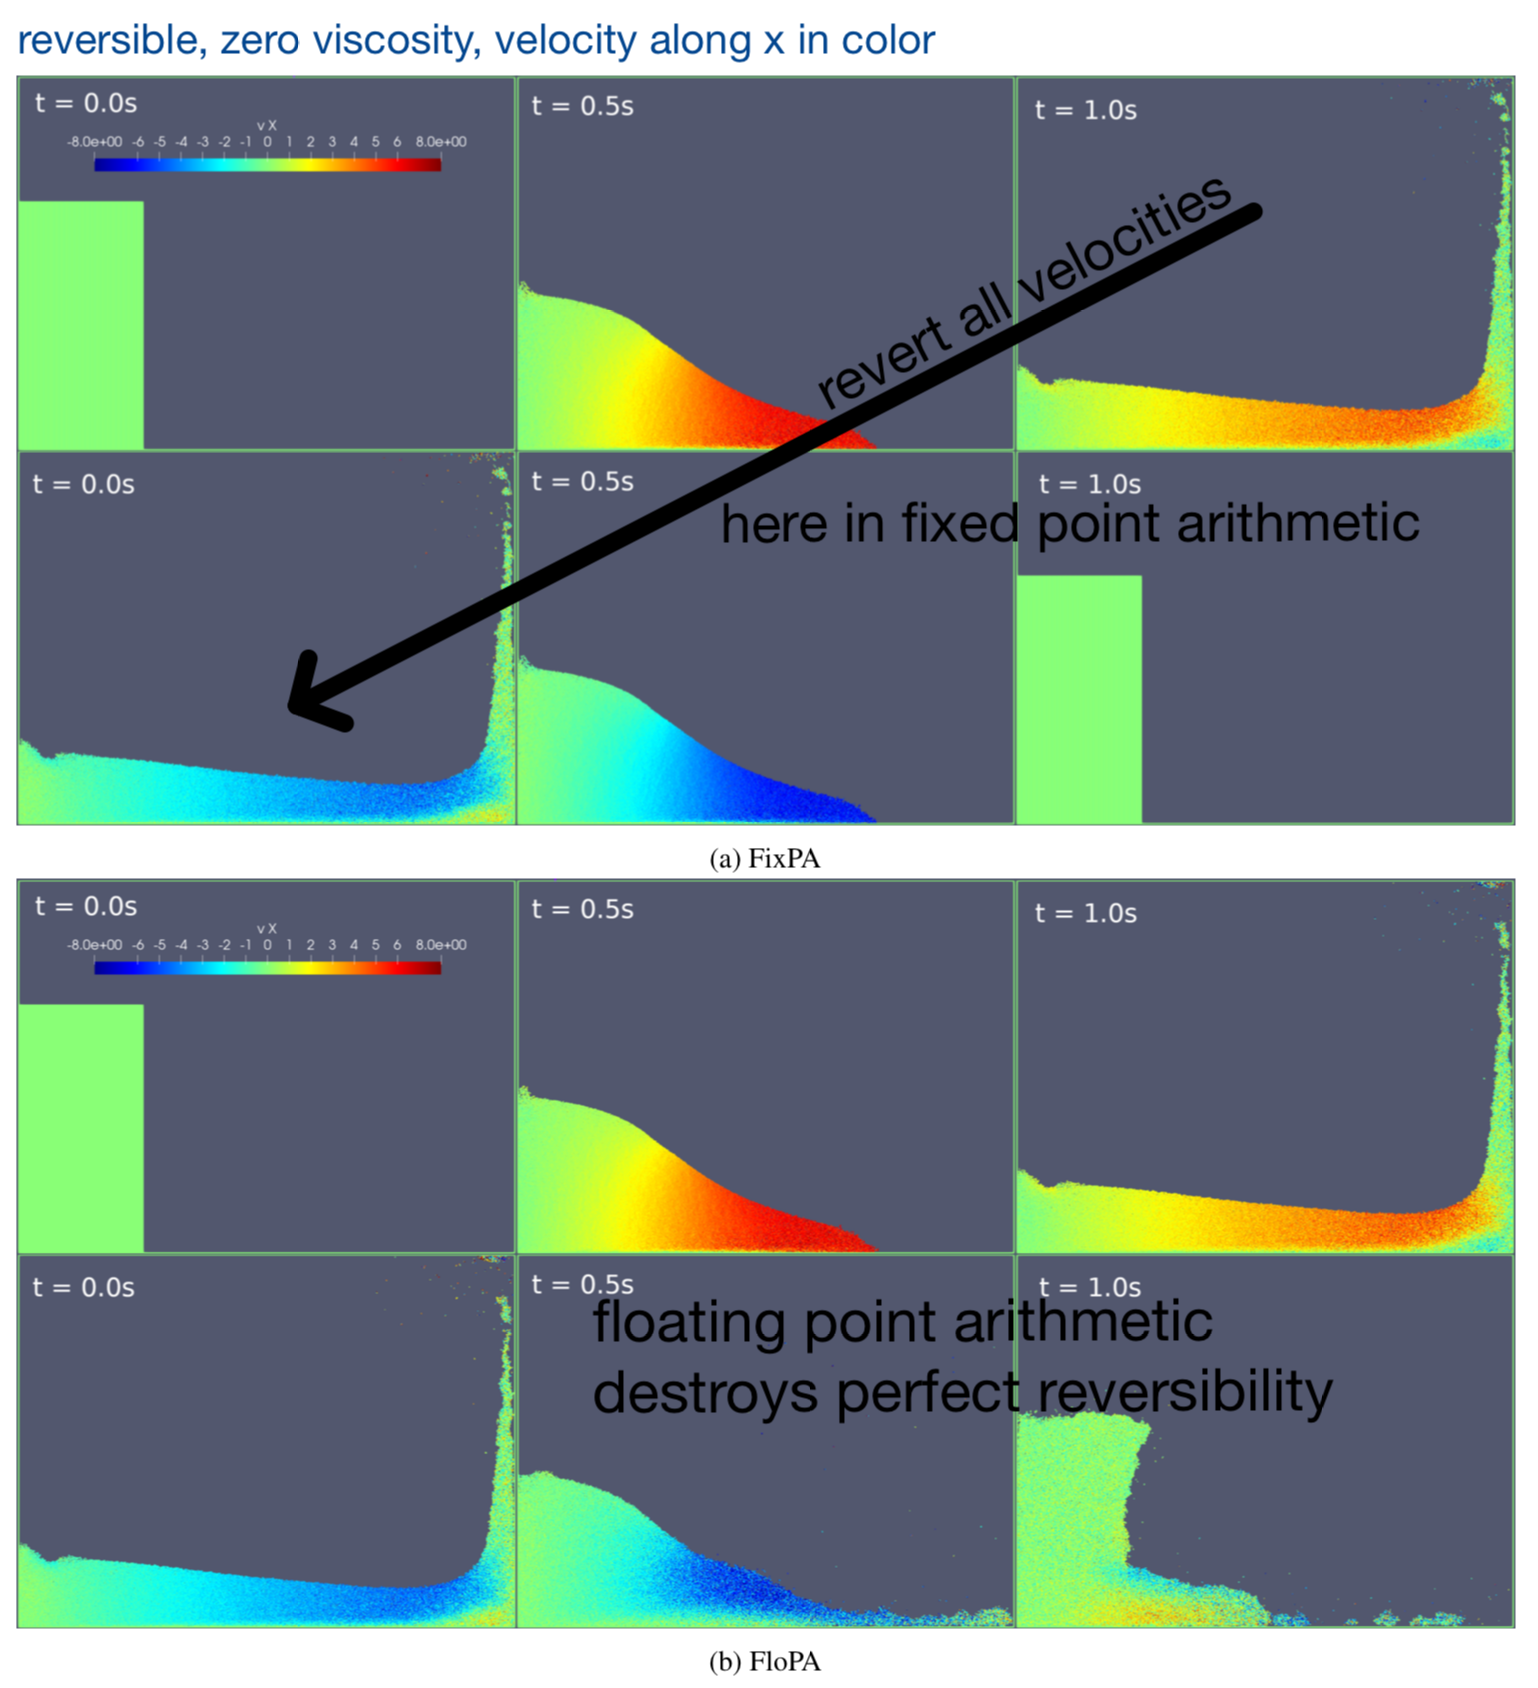
\includegraphics[width=0.8\textwidth]{figures/reversible_dam3.png}
    \caption{Reversible SPH simulation without viscosity at the example of a breaking dam. In floating-point arithmetic this reversible behavior is broken. Being in an initial state leading back to the \textit{dam} is very unlikely so even slight deviations will make us not go back to the dam.}
    \label{fig:reversible_dam}
\end{figure}

\yellowbox{\textbf{Note the different levels at play:} The SPH-particles are artificial in that they describe the fluid not the fluid particles. So while the SPH-particles start out resting, there is still temperature and pressure. However, in the dam experiment (fig. \ref{fig:reversible_dam}) (and generally) the SPH particles themselves thermalize to a Boltzmann distribution (they start out in non-equilibrium), fitting to the equilibrium Boltzmann entropy (although we do not add any heat, Boltzmann entropy of the SPH-particles (\textbf{based on their phase space distribution}) increases as we go from non-equilibrium to equilibrium). Note that this is not the same as the specific thermodynamic entropy of the fluid, as previously described.}

\subsection{Notes on the conservative formulation using Lagrange multipliers}
Starting with the Lagrangian for inviscid, compressible flow
\begin{equation}
    \mathcal{L}=\int \rho\left\{\frac{1}{2} v^2-u(\rho, s)\right\} d^3 r
\end{equation}
the SPH equation with $s = \text{const.}$ follows from the Lagrange equation
\begin{equation}
    \frac{d}{d t} \frac{\partial \mathcal{L}}{\partial \vec{v}}-\frac{\partial \mathcal{L}}{\partial \vec{r}}=0
\end{equation}
(for variable smoothing length $h$ under the constraint (Lagrange multiplier) $\rho_j h_j^3 = \text{const.}$) as
\begin{equation}
    \frac{d \vec{v}_i}{d t}=-\sum_{j=1}^{N_i} m_j\left\{\frac{1}{f_i} \frac{p_i}{\rho_i^2} \vec{\nabla}_i W\left(r_{i j}, h_i\right)+\frac{1}{f_j} \frac{p_j}{\rho_j^2} \vec{\nabla}_i W\left(r_{i j}, h_j\right)\right\}, \quad f_i=\left[1+\frac{h_i}{3 \rho_i} \frac{\partial \rho_i}{\partial h_i}\right]
\end{equation}
From the symmetries of the Lagrangian it follows that energy, specific thermodynamic entropy, linear and angular momentum are conserved.

\subsection{Further improvements}
Ideas for improvement are
\begin{itemize}
    \item it may be more physical to move particles with a smoothed flow velocity
    \item ...
\end{itemize}

\subsection{Advantages and Disadvantages of SPH}
% table with advantages and disadvantages of SPH
Advantages and disadvantages of SPH are summarized in table \ref{tab:advantages_disadvantages_sph}.

\begin{table}[!htb]
    \centering
    \begin{tabular}{p{0.45\textwidth}|p{0.45\textwidth}}
        \textcolor{green1}{Advantages} & \textcolor{red1}{Disadvantages} \\
        \hline \\
        \begin{itemize}
            \item versatile and simple
            \item avoids numerical diffusion issues arising when advection is not aligned with the mesh
            \item automatically adaptive resolution, can cover large ranges in density and space
            \item excellent conservation properties (energy, linear and angular momentum, not guarantueed in Eulerian codes)
            \item inherent mass conservation
            \item Galilean invariant and free from advection errors
            \item can deal with complicated geometries as mesh-free
            \item simple and transparent codes
            \item very robust
            \item as a particle scheme it is good for describing the transition from gaseous to stellar dynamical systems (e.g. formation of stellar clusters)
        \end{itemize} &
        \begin{itemize}
            \item limited accuracy in multi-D flow
            \item The number of neighboring particles (based on the neighbors positions we calculate the density and then equations of motion at the particle of interest) in SPH is far greater than the number of neighboring nodes in mesh based methods
            \item low density regions are more poorly resolved
            \item poorly handles shocks
            \item noise as of discrete sums over limited neighbor set
            \item jitter develops
            \item fluid instabilities arcoss contact discontinuities are problematic such as Kelvin helmholtz instabilities
            \item artificial viscosity limits the Reynolds number which can be reached
            \item low convergence rate \footnote{Convergence in the SPH case means that with increasing number of SPH particles we approach the correct fluid behavior.}
            \item approximation of boundary conditions can be difficult
            \item formation of voids
            \item free surfaces can be problematic (density underestimated there)
            \item magnetic fields are hard to handle (problems with stability and $\vec{\nabla} \cdot \vec{B} = 0$ requirement)
        \end{itemize} \\
    \end{tabular}
    \caption{Advantages and disadvantages of SPH.}
    \label{tab:advantages_disadvantages_sph}
\end{table}

\subsection{Outlook: Machine-learning enhanced multiscale-physics SPH simulation}
Consider a SPH simulation of the Milky Way. In the N-body/SPH simulation
individual SPH particles represent a clump of dark matter, gas or a group of stars.

\greenbox{It is desirable do use particles with as small mass as possible, the current 
state of the art is $10^3 M_{\odot}$\footnote{$1 M_{\odot}$ is the mass of the sun.}. \cite{hirashima2023}
push for a model with resolution $~1 M_{\odot}$ for galaxy formation and evolution.}

\problem{Such high resolution galaxy evolution simulations consider multi-scale physics - 
a tiny fraction of short timescale regions (e.g. Supernovae) becomes the bottleneck
for large scale parallel computation due to \textbf{Ahmdals law} (discussed later).}

\idea{Replace the direct simulation of short time-step regions with a \textit{surrogate} machine learning model (that can directly do a large physically adequate time-step)
that learns from supernova simulations in turbulent gas clouds.}

\problem{The machine learning model (e.g. U-Net) needs a voxel (grid) representation. Density temperature
and 3D velocity can e.g. be represented as $5$ scalar fields on a 3D grid.}

\idea{Based on the SPH particles we can construct a 3D grid representation that we can feed
into our ML model (e.g. U-Net) in the respective regions. After doing the larger timestep with 
U-Net, we get back from the Eulerian voxel / field representation to SPH-particles by Gibbs-Sampling\footnote{A technique for generating samples of the marginals based on the conditional distributions in a multivariate setting.
Consider e.g. we have a probability distribution for particles in $3$D, $p(x,y,z)$. Imagine that one can easily
sample from the conditionals but not easily from the known joint distribution. \textbf{Gibbs sampling}:
\begin{enumerate}
    \item Choose an initial state $(x_0, y_0, z_0)$
    \item Do an iteration with $t = 1,2,\dots,N$:
    \begin{enumerate}
        \item Sample $x^{(t)}$ from $p(x|y^{(t-1)}, z^{(t-1)})$
        \item Sample $y^{(t)}$ from $p(y|x^{(t)}, z^{(t-1)})$
        \item Sample $z^{(t)}$ from $p(z|x^{(t)}, y^{(t)})$
    \end{enumerate}
\end{enumerate}
Where the conditionals just follow from the joint distribution $p(x,y,z)$ by plugging in the calculated values for the other variables. A burn in of $\sim 1000$ iterations is often used.
\textbf{Note that a standard \textit{global} Metropolis Hastings algorithm can get us (multivariate) samples from the total joint distribution directly, not by sampling from the marginals seperately.}
The rough rationale behind Gibbs sampling is that it might be easier to propose updates to one variable at a time than to all simultaneously as in such a Metropolis Hastings algorithm (Gibbs sampling is also
a special case of a Metropolis Hastings algorithm).
} (a Marcov Chain Monte Carlo method).}

\pagebreak